%%%%%%%%%%%%%%%%%%%%%%%%%%%%%%%%%%%%%%%%%%%%%%%%%%%%%%%%%%%%%%%%%%
%%%%%%%% ICML 2012 EXAMPLE LATEX SUBMISSION FILE %%%%%%%%%%%%%%%%%
%%%%%%%%%%%%%%%%%%%%%%%%%%%%%%%%%%%%%%%%%%%%%%%%%%%%%%%%%%%%%%%%%%

% Use the following line _only_ if you're still using LaTeX 2.09.
%\documentstyle[icml2012,epsf,natbib]{article}
% If you rely on Latex2e packages, like most moden people use this:
\documentclass{article}

% For figures
\usepackage{graphicx} % more modern
%\usepackage{epsfig} % less modern
\usepackage{subfigure} 

% For citations
\usepackage{natbib}

% For algorithms
\usepackage{algorithm}
\usepackage{algorithmic}

% As of 2011, we use the hyperref package to produce hyperlinks in the
% resulting PDF.  If this breaks your system, please commend out the
% following usepackage line and replace \usepackage{icml2012} with
% \usepackage[nohyperref]{icml2012} above.
\usepackage{hyperref}

% Packages hyperref and algorithmic misbehave sometimes.  We can fix
% this with the following command.
\newcommand{\theHalgorithm}{\arabic{algorithm}}

% Employ the following version of the ``usepackage'' statement for
% submitting the draft version of the paper for review.  This will set
% the note in the first column to ``Under review.  Do not distribute.''
\usepackage[accepted]{icml2012} 
% Employ this version of the ``usepackage'' statement after the paper has
% been accepted, when creating the final version.  This will set the
% note in the first column to ``Appearing in''
% \usepackage[accepted]{icml2012}


% The \icmltitle you define below is probably too long as a header.
% Therefore, a short form for the running title is supplied here:
\icmltitlerunning{Structure Learning and Implementation in Bayesian Network}

\begin{document} 

\twocolumn[
\icmltitle{Structure Learning and Implementation in Bayesian Network}

% It is OKAY to include author information, even for blind
% submissions: the style file will automatically remove it for you
% unless you've provided the [accepted] option to the icml2012
% package.
\icmlauthor{Dingxin Yu}{dingxin.yu@postgrad.manchester.ac.uk}
\icmladdress{School of Computer Science, The University of Manchester}


% You may provide any keywords that you 
% find helpful for describing your paper; these are used to populate 
% the "keywords" metadata in the PDF but will not be shown in the document
\icmlkeywords{machine learning}

\vskip 0.3in
]

\begin{abstract} 
This work is aimed to evaluate performance of Bayesian network for different directed acyclic graphs (DAGs) and explore Bayesian network property. Implementation and all experiments are accomplished in Java and Matlab environment using different test data sets in three categories. Experiments including how the likelihood and log-likelihood measure of Bayesian Network differs as the number of training data set changes, scoring function and fill distribution strategy in Bayesian network. Besides, the performances of different Bayesian network DAGs will be evaluated against various data set as well.
\end{abstract} 

\section{Introduction}
\label{submission}

In order to reach conclusions based on current information. A general approach for this purpose is given by probabilistic graphical models is allowing interpretable models to be constructed and then processed by reasoning algorithms by corresponding different models. 
Due to uncertainty of most real-world application, it is almost impossible to manually creating a model from various data. In this case, these probabilistic models can be learned automatically from data by using different algorithms. A variety of models discussed by probabilistic graphical models including spanning Bayesian networks, discrete and continuous models, undirected Markov networks, and extensions to deal with dynamical systems and relational data\cite{prob}. Bayesian network will be mainly discussed in later chapters with corresponding experiments.

Bayesian networks is a compact representation of conditional dependency relation between random variables. It consists of a graph and conditional probability tables. The graph is set of nodes that represents a set of random variables. Each variable has a finite set of values. Set of directed edges that represent dependency relationship between the corresponding random variables. Bayesian Network is a graph augmented with Conditional Probability Tables(CPTs) whereas vertices represent random variables and edges represent dependency between random variables.

This article consists mainly of introduction, background, experiments, analyses and conclusion. Bayesian network structure and its measuring properties are described in background section. In addition, techniques used during investigation and outlines are listed. All experimental work including performance tests are described and presented in graphs. Results will be analysed in details.  Besides, conclusions and future concern are included as well.

\section{Background}

Numbers of methodologies are included in this project.

\subsection{Markov Blanket and Value Elimination}
Markov blanket and value elimination algorithm are two foundations in Bayesian network. A variable in a Bayesian network is conditionally independent from all other, given its Markov blanket. Markov blanket of a node X consists of parents of X, children of X and parents of children of X\cite{value}. Value elimination is an algorithm for Bayesian network inference\cite{markov}. The idea of value elimination algorithm is to use conditional independence to reduce the number of calculation combinations. That is also considered as one of the most important advantages of Bayesian network. 

\begin{figure}[ht]
\vskip 0.2in
\begin{center}
\centerline{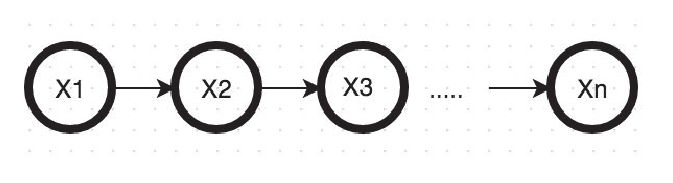
\includegraphics[width=\columnwidth]{rChain}}
\caption{Random Chain Structure}
\label{rChain}
\end{center}
\vskip -0.2in
\end{figure} 

\begin{algorithm}[tb]
   \caption{Value Elimination}
   \label{alg:value}
\begin{algorithmic}
   \STATE {\bfseries Input:} A Bayesian network with variables $X_1,...,X_m$ and an elimination order.
   \STATE Initialize $noChange = true$.
   \FOR{$i=m$ {\bfseries to} $1$}
   \STATE Remove all the factors that mention $X_i$
   \STATE Multiply those factors, getting a value for each combination of mentioned variables.
   \STATE Sum over $X_i$
   \STATE Put this new factor into the factor set
   \ENDFOR
\end{algorithmic}
\end{algorithm}

For example, by using those terminologies, if there is a n binary variable $X_1, X_2.....X_n$ and we want to computer probability of $X_n$ equals 1, then in general we have to marginalize the probability over $n-1$ variables which is sum of $2^{n-1}$ elements. However, if conditional independence relationship can be represented in Bayesian network in Figure~\ref{rChain}.

Each summation can be computed first by value elimination algorithm. Probability of $X_n$ equals 1 can be computed with $n - 1$ rather than $2^{n-1}$ summations. 

\subsection{Goodness of Fit Measure}
Likelihood is used to test which Bayesian network has better goodness of fit. Generally, a higher likelihood or log-likelihood represents better Bayesian network. It means this data set is more likely to have occurred under this model.

\textbf{Likelihood:}$P(Data|Model)$
\begin{eqnarray}
&=& \prod_{i} P(Data_{i}|Model)\\
&=&\prod_{i}\prod_{j} P(N_{i}^{j}|Parent(N^{j}), Model)
\end{eqnarray}
\textbf{Log-Likelihood:}$P(Data|Model)$
\begin{eqnarray}
&=&log(\prod_{i}\prod_{j} P(N_{i}^{j}|Parent(N^{j}), Model))\\
&=&\sum_{i}\sum_{j}log(P(N_{i}^{j}|Parent(N^{j}), Model)))
\end{eqnarray}


The two likelihoods are linked very simply. Basically, the log-likelihood is just the log of the likelihood calculation.  However, which one gives a better way to measure Bayesian network will be experimented in later chapter.

\subsection{Scoring Function}
Due to overfitting issue, simple structure is preferred. In other word, a simpler network with higher log-likelihood is better. And in this case, another terminology named scoring function\cite{score}is a way to measure with following arithmetic expression. 

$Score = log(P(Data|Model)) - C*E$

Where E represents total number of elements in the CPT and constant C is a parameter to trade-off goodness of fit and simplicity of the network. Corresponding experiments designed for scoring function with constant C.

\subsection{Bayesian Network With Different DAGs}
There are various of different DAGs in Bayesian network. Three typical DAGs are chosen for this project which are No Edge, Random Chain and Best Tree.

No Edge is the simplest with smallest complexity among DAGs. In other word it is an empty graph. 

\begin{figure}[ht]
\vskip 0.2in
\begin{center}
\centerline{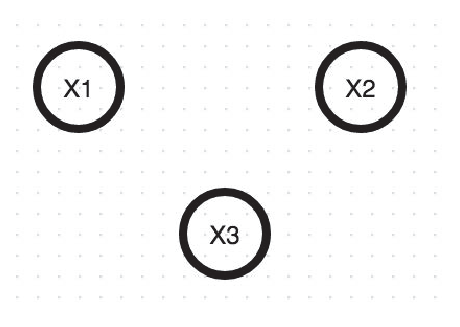
\includegraphics[width=\columnwidth]{noEdge}}
\caption{No Edge Structure}
\label{noEdge}
\end{center}
\vskip -0.2in
\end{figure} 

Random chain can be generated by choosing random ordering of the vertices, e.g., $V_1,....,V_n$. Create a chain, i.e., Vi is the only child of $V_{i-1}$.

\begin{figure}[ht]
\vskip 0.2in
\begin{center}
\centerline{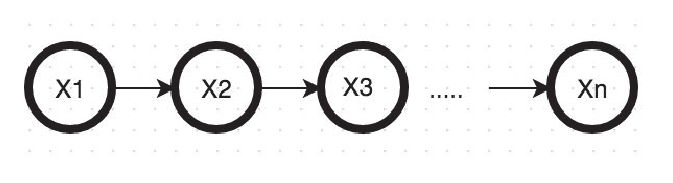
\includegraphics[width=\columnwidth]{rChain}}
\caption{Random Chain Structure}
\label{raChain}
\end{center}
\vskip -0.2in
\end{figure} 

Best tree is a fully connected graph G, i.e., there is always en edge between each pair of vertices. Weigh of the edges computed by mutual information between each pair of random variables by following formula. It also known as minimum weight spanning tree.
$MI(A,B)$
$=\sum P(A=a, B=b)log(\frac{P(A=a, B=b)}{P(A=a) * P(B=b)})$

\begin{figure}[ht]
\vskip 0.2in
\begin{center}
\centerline{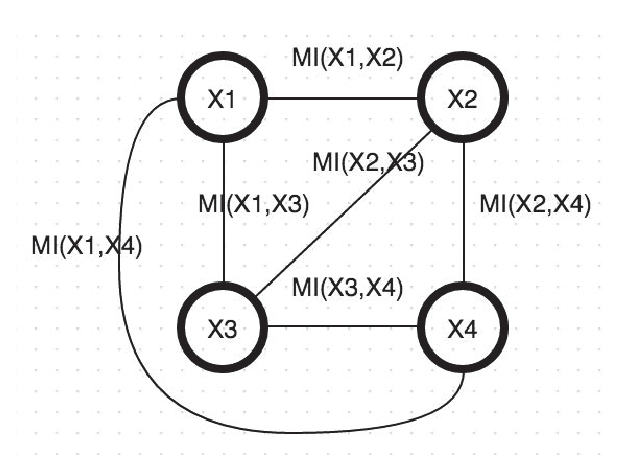
\includegraphics[width=\columnwidth]{btree}}
\caption{Best Tree Structure}
\label{btree}
\end{center}
\vskip -0.2in
\end{figure} 

A numbers of experiments are designed for structure evaluation against different kind of data sets by the same search strategy with different initial DAGs.


\textbf{Search possible structures}
\begin{itemize}
\item S - All possible DAGs with vertices as random variables
\item A - add or remove edge, reverse direction
\item Deterministic
\item Goal - Stop when score reaches limit or after certain time.
\end{itemize}
In this case, suppose there is no missing data in data set.

\subsection{Missing Data Handling }
For a given data from Table~\ref{data}, assume each experimental data is independent.

$P(Data, H|Model)$
\begin{eqnarray}
&=&P(Data_3, H|Model)\\
&=&P(A|~B, Model)\\
&=&P(~B|A, Model)P(A|Model)
\end{eqnarray}

CPTs can be computed by counting with expected counts for H. A probability of H, will be generated by thoes method.
\begin{table}[t]
\caption{Missing Data Example} 
\label{data}
\vskip 0.15in
\begin{center}
\begin{small}
\begin{sc}
\begin{tabular}{lcccr}
\hline
\abovespace\belowspace
Exp & A & B \\
\hline
\abovespace
1    & 1 & 1& \\
2	 & 0 & 1& \\
3    & H & 0&  \\
\hline
\end{tabular}
\end{sc}
\end{small}
\end{center}
\vskip -0.1in
\end{table}


\section{Experiments}

It is assumed that all variables are binary variables. The value are either 0 or 1 for all experiments.

\subsection{Compare Log-likelihood and Likelihood}
The training data sets for this part are the txt files whose names start with CPTNoMissingData. The format of each data file is:
The first line contains two numbers separated by a white space. The first number is the number of nodes in the Bayesian Network. 
The second number is the number of data in the file. Let’s denote the number of nodes as K and the number of data as N. Each line at line 2 to K+1 represents a node of the Bayesian Network and its parents. Each line contains one or more words, separated by a white space. The first word represents the name of the node, while the rest represents the names of the node’s parents. For example, “A B C” means Node B and C are the parents of node A. 

Each line at line $K+2$ to $K+N+1$ represents the data, in the same order the nodes are written. For instance, in CPTNoMissingData-d1.txt, each line of data represents the value of A B C.
Table~\ref{likeli-table} are concluded from result file cpt-CPTNoMissingData-dx-log and cpt-CPTNoMissingData-dx. Last Line is the log-likelihood of the data given the Bayesian Network model.

\begin{table}[t]
\caption{Likelihood and Log-likelihood}
\label{likeli-table}
\vskip 0.15in
\begin{center}
\begin{small}
\begin{sc}
\begin{tabular}{lcccr}
\hline
\abovespace\belowspace
Data set & Log-likelihood & Likelihood \\
\hline
\abovespace
d1    & -10.54193498725965 & 0.0& \\
d2	  & -57.064187498416835 & 0.0& \\
d3    & -10320.88431900996 & 0.0&  \\
\hline
\end{tabular}
\end{sc}
\end{small}
\end{center}
\vskip -0.1in
\end{table}
\textbf{\texttt{Log base is 10 for this experiment.}}

\subsection{Change Constant C in Scoring Function}
The training data sets for this experiment are the txt files whose names start with noMissingData. 
The format of each data file is the same as the input format for experiment 3.1, but without the parents’ information, i.e.: The first line contains two numbers separated by a white space. The first number is the number of nodes in the Bayesian Network. The second number is the number of 2 data in the file. The number of nodes are donated as K and the number of data as N. 

The second line represents the names of the nodes, separated by a white space. 

Each line at line 3 to $N+2$ represents the data. 

Results are generated by using different constant C. Result files for this experiment are result-ConstantCompare-bn-noMissingData Last Line consists of two number separated by a white space. The first number is the log-likelihood of the data given the Bayesian Network model. The second number is the score of the Bayesian Network. Bayesian network model structure and corresponding CPT for each node are presented above log-likelihood and score.

\begin{figure}[ht]
\vskip 0.2in
\begin{center}
\centerline{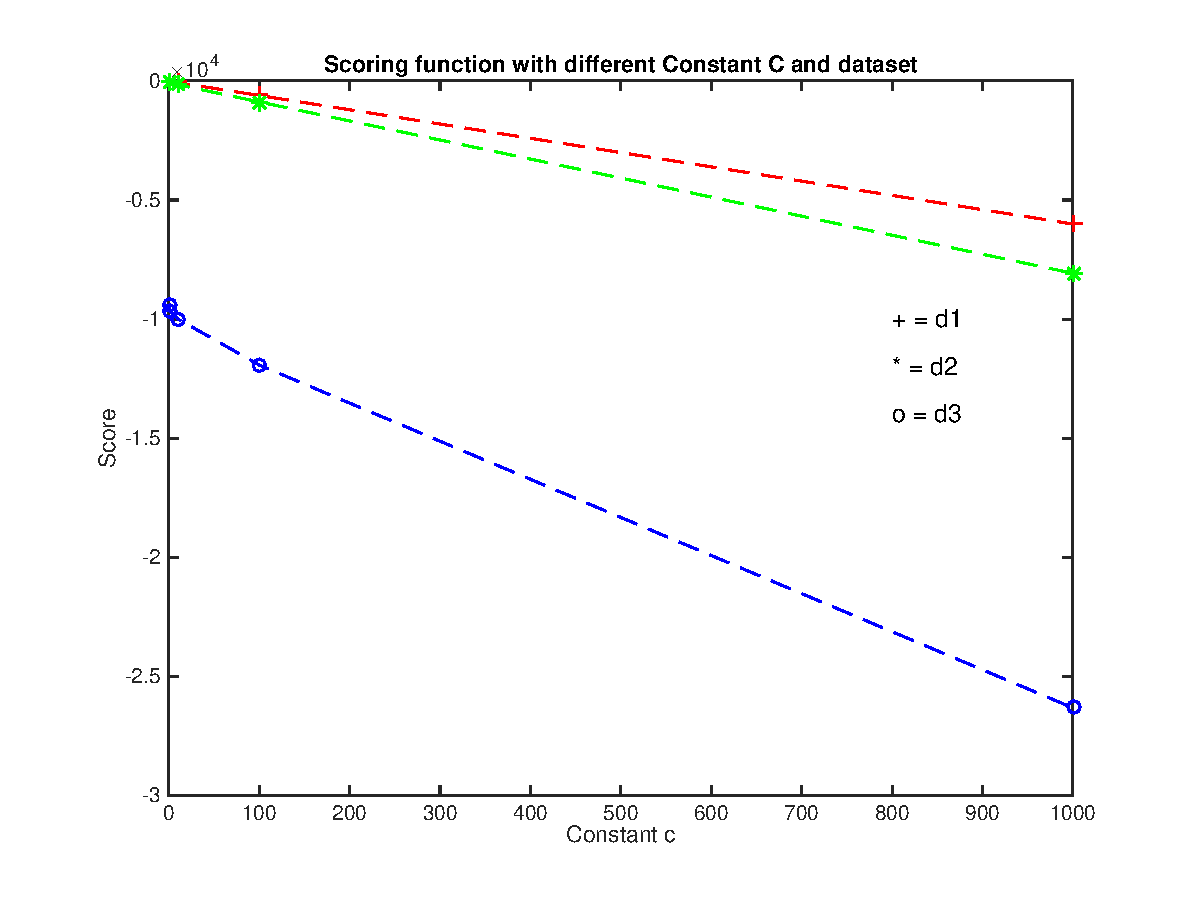
\includegraphics[width=\columnwidth]{constant_comp}}
\caption{Score with different constant C.}
\label{constant_Comp}
\end{center}
\vskip -0.2in
\end{figure} 

\begin{figure}[ht]
\vskip 0.2in
\begin{center}
\centerline{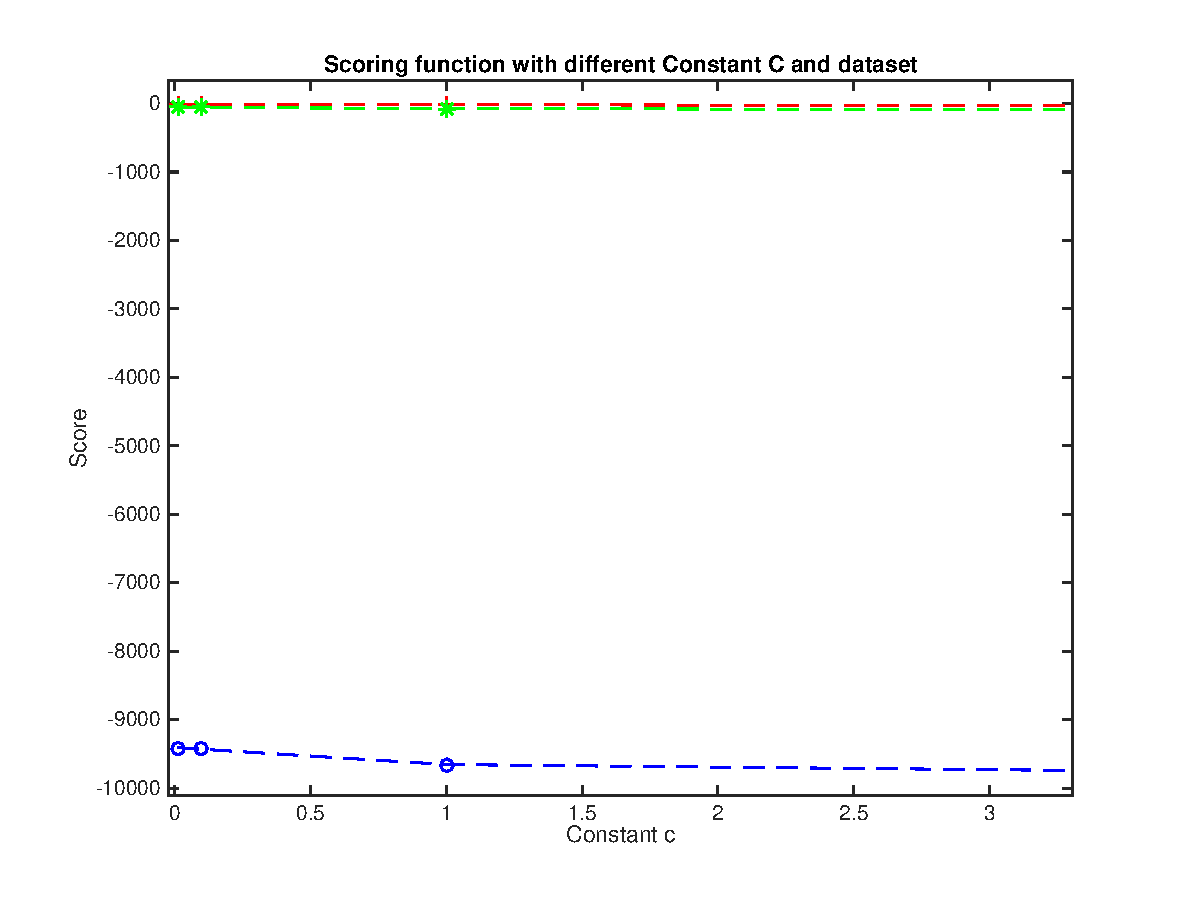
\includegraphics[width=\columnwidth]{constant_compd}}
\caption{C with value of 0.01, 0.1, 1.}
\label{constant_Compd}
\end{center}
\vskip -0.2in
\end{figure} 

\subsection{Compare Different Initial DAGs}
The training data sets for this experiment are the same files as experiment 3.2. And some proper constant C and threshold are set for different data set. Three minutes are time limitation for each data set and corresponding DAGs in this experiment. Table~\ref{NoEdge}, \ref{RandomChain} and \ref{BestTree} are generated from result file starting with noEdge, rChain and btree. Result format is the same as experiment 3.2. Same constant C is set for corresponding data set.

\begin{table}[t]
\caption{No Edge Structure}
\label{NoEdge}
\vskip 0.15in
\begin{center}
\begin{small}
\begin{sc}
\begin{tabular}{lcccr}
\hline
\abovespace\belowspace
No Edge & Log-likelihood & Score \\
\hline
\abovespace
d1    & -10.6916372 & -40.6916372& \\
d2	  & -60.5681333 & -110.568133& \\
d3    & -9457.04647 & -9518.04647&  \\
\hline
\end{tabular}
\end{sc}
\end{small}
\end{center}
\vskip -0.1in

\caption{Random Chain Structure}
\label{RandomChain}
\vskip 0.15in
\begin{center}
\begin{small}
\begin{sc}
\begin{tabular}{lcccr}
\hline
\abovespace\belowspace
Random Chain & Log-likelihood & Score \\
\hline
\abovespace
d1    & -10.6916372 & -40.6916372& \\
d2	  & -60.5681330 & -110.568133& \\
d3    & -9448.46799 & -9517.46799&  \\
\hline
\end{tabular}
\end{sc}
\end{small}
\end{center}
\vskip -0.1in

\caption{Best Tree Structure}
\label{BestTree}
\vskip 0.15in
\begin{center}
\begin{small}
\begin{sc}
\begin{tabular}{lcccr}
\hline
\abovespace\belowspace
Best Tree & Log-likelihood & Score \\
\hline
\abovespace
d1    & -10.6916372 & -40.6916372& \\
d2	  & -60.5681330 & -110.568133& \\
d3    & -9454.58890 & -9499.58890&  \\
\hline
\end{tabular}
\end{sc}
\end{small}
\end{center}
\vskip -0.1in
\end{table}

\subsection{Calculate Missing Data Using Fill In Distribution}
The training data sets for this part are files that start with someMissingData. The format of each data file is the same as the input format for experiment 3.2 and experiment 3.3, but each data input may have a value of 0, 1, or H1/H2/.../HM, where Hi means missing data and M is the number of missing data. 

In this experiment, missing data separated by a white space, where M is the number of missing data. The first word is the name of the missing data (e.g., H1, H2, etc.). The second word is the probability that the missing data has value 1. For example, if $P(H1 | Data, Model) = 0.6$, then the output will be: “H1 0.6”.

Table~\ref{missing-data} shows log-likelihood and score for best tree structure with some missing data set.

\begin{table}[t]
\caption{Score for Some Missing Data in Best Tree Structure}
\label{missing-data}
\vskip 0.15in
\begin{center}
\begin{small}
\begin{sc}
\begin{tabular}{lcccr}
\hline
\abovespace\belowspace
Data set & Log-likelihood & Score \\
\hline
\abovespace
d1    & -10.775436 & -25.775436& \\
d2	  & -62.621634 & -97.621634& \\
d3    & -9435.40280 & -9594.40280&  \\
\hline
\end{tabular}
\end{sc}
\end{small}
\end{center}
\vskip -0.1in
\end{table}

By using of fill in distribution strategy, missing data are calculated in file bn-someMissingData for corresponding data set.

\section{Analysis}
\subsection{Compare Log-likelihood and Likelihood}
According to Table~\ref{likeli-table}, likelihood is 0.0 for all three training sets. The reason why it is 0.0 is because double limitation in Java. However, likelihood should trend to be 0 for the increasing number of data or node in Bayesian network. Log-likelihood is therefore better in measuring Bayesian network. With a higher value of log-likelihood means the corresponding data set is more likely to have occurred under this model .


\subsection{Change constant C in Scoring Function}

Several positive constant C (0.01, 0.1, 1, 10, 100, 1000) are chosen for scoring function. The reason why C cannot be negative is, it will actually end up increasing the score as the Bayesian network get more complex.
According to Figure~\ref{constant_Comp} and Figure~\ref{constant_Compd}, it is hard to distinguish score between data set 1 and data set 2 when C is a small value by using same Bayesian network structure. 
Thus, larger C is suitable in simpler Bayesian network structure. And smaller C is better for complex structure, due to the consideration of accuracy. 

\subsection{Compare different Initial DAGs}
According to Table~\ref{NoEdge}, Table~\ref{RandomChain} and Table~\ref{BestTree}, all three different structure generated the same score for data set1 and data set2 within three minutes. Nevertheless, No Edge and Random Chain have less ram cost than Best Tree in processing with data set1 and data set2.However, with the increasing number of samples and node in Bayesian network, Best Tree got the highest score among three DAGs. 

In conclusion, under proper constant C for scoring function, Best Tree is proper structure for complicated node relationship with Bayesian network, No Edge is better for simple node relationship and small data set. Random Chain is an alternative choice if node relationship is unknown.

\subsection{Missing Data Handling}
Fill in distribution is a good solution to missing data. The result file simply shows the probability that the missing data has value 1. After replacing 1 or 0 by using of probabilities from result file, result of Bayesian network would not change significantly. However, if the percentage of missing data is not very high, Bayesian network can still generate reasonable result by ignoring those missing data. In this case, cost of time and RAM will be reduced. 

\section{Conclusions} 
This work is aimed to evaluate performance of Bayesian network for different DAGs and explore Bayesian network property. 

Experiments 3.1 and 3.2 are focusing on model evaluation properties including how the likelihood and log-likelihood measure of Bayesian Network differs as the number of training dataset changes and scoring function with different constant C. The value of log-likelihood will increase, as the number of node relationship increase. But simple Bayesian network structure is preferred, due to consideration of over-fitting. Score function is therefore involved in this case. Constant C could be treated as balance constant between accuracy and model complexity.

Experiment 3.3 shows the performances among different DAGs. A fully connected graph is better for complex CPT relationship whereas an empty graph suits simple data set very well.

In addition, fill in distribution strategy is well explained with support data set in Experiment 3.4.
 
Furthermore, there are some limitations and future considerations for this project. The details are listed below.
\begin{itemize}
\item Should use big decimal instead of double in Java. In this case, value of likelihood would not be 0.0.
\item Should use natural log instead of log base 10. It might be more reasonable.
\item Time limitation should be smaller for simple data set. More straightforward sight in comparing different structure.
\item Should have implementation on ignoring strategy. 
\end{itemize}

In conclusion, all above discussed properties and various structures make Bayesian networks become increasingly being used to model environmental systems, particularly in concluding information from different data sources and handling missing data and uncertainty.


\bibliography{example_paper}
\bibliographystyle{icml2012}

\end{document} 


